\chapter{Résultats}


\paragraph{Performance théorique:} Suite à l'apprentissage du réseau de neurone, nous avons obtenu une précision de 59.0\% sur les données d'entrainement,
de 58.9\% sur les données de tests avant quantization et 58\% après.
La matrice de confusion nous permet de voir que les chants ont été globalement 
bien appris avec une majorité de vrais positifs pour la plupart des classes cf: Figure \ref{graph:confusion_matrix1}.
Les classes présentant le plus de confusion sont les classes 0, 3, 4 et 5 avec un maximum de confusion pour la classe 3.
Ces classes représentent les oiseaux suivants :

\begin{itemize}
  \item 0: Alauda Arvensis
  \item 3: Emberiza Cirlus
  \item 4: Emberiza Citrinella
  \item 5: Falco Tinnunculus
\end{itemize}

\begin{figure}[!ht]
  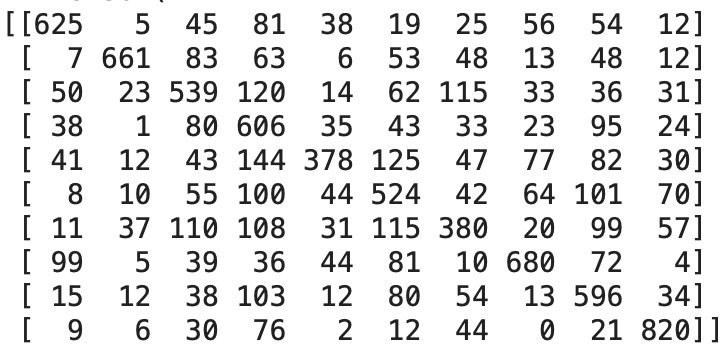
\includegraphics[width=0.5\textwidth]{confusion_matrix1}
  \centering
  \caption{Matrice de confusion}
  \label{graph:confusion_matrix1}
\end{figure}

\paragraph{Performance expérimentale:} Pour tester nos résultats nous avons déployé le réseau de neurone sur la carte Nucleo à l'aide 
de l'IDE Arduino. Pour cela nous avons utilisé le même projet Arduino que dans le Lab 5, lors de la réalisation du CNN à partir du
jeu de donnée Google Speech Commons. Nous avons modifié le programme pour qu'il n'écrive dans la sortie Serial que lorsque la valeur prédite maximale
est supérieure à 8000. Cela permet de n'afficher que les résultats étant plus en faveur d'une classe que d'une autre.
Nous avons ensuite testé le modèle en jouant sur les haut-parleurs des sons n'étant pas présents dans notre jeu de données.

Nous avons pu remarquer que lorsque qu'un chant d'oiseau est joué et qu'un résultat est donné, celui-ci est le bon dans la majorité des cas.
Cependant, nous recevons parfois des résultats en présence de bruits forts, alors qu'aucun bruit d'oiseau n'est joué. 
Cela peut être dû à la présence dans notre jeu de données d'échantillons de bruits de fond, où aucun oiseau ne peut être entendu.

\paragraph{Mémoire}
\paragraph{Latence}
\paragraph{Energie}
• Analysis of the result of your project on the following criteria
o Performance (accuracy on train, test and on real data after quantization)
o Memoryfootprint
o Latency
o Energy consumption and battery lifetime analysis (provide assumptions of your
estimation)

